\documentclass[11pt,a4j]{jarticle}
\usepackage[dvipdfmx]{graphicx}
\usepackage{multirow}

\title{Newcomer Task}
\author{Shinnosuke Matsuo}
\date{April 2020}

\begin{document}

\maketitle
今回の新人課題では,以下の3つの課題を選択した.
\begin{itemize}
  \item Basic Image Processing
  \item Medical Image Classification
  \item Time Series Classification
\end{itemize}

ソースコードは,https://github.com/matsu-shin/assignment2020に公開している.各課題のフォルダの中の.jpynbファイルにコードが格納されている.

\section{Basic Image Processing}

\subsection{Python+OpenCVのプログラミング環境構築}
Fig\ref{output_0}に示すように,PythonコードをOpenCV(cv2)のバージョンが出力されていることから,Python+OpenCVのプログラミング環境の構築ができていることがわかる.
\begin{figure}[ht]
	\centering
	\includegraphics[width=\linewidth]{../1_BasicImageProcessing/output/output_0.jpg}
	\renewcommand{\figurename}{Fig}
	\caption{Python+OpenCV Environment}
	\vspace{1cm}
	\label{output_0}
\end{figure}

\subsection{Numpyを使った行列の四則演算}
Fig\ref{output_1}に示すように,行列A,Bを定義し,それらを用いて四則演算を行った.
\begin{figure}[ht]
	\centering
	\includegraphics[width=\linewidth]{../1_BasicImageProcessing/output/output_1.jpg}
	\renewcommand{\figurename}{Fig}
	\caption{Four Arithmetic Operations by Numpy}
	\label{output_1}
\end{figure}

\subsection{画像の表示,縮小拡大,回転,二値化}
このセクションでは,Fig\ref{LysGracieux}のリスグラシューの画像を用いて,表示,縮小拡大,回転,二値化を行っていく.
\begin{figure}[ht]
	\centering
	\includegraphics[width=5cm]{../1_BasicImageProcessing/data/LysGracieux_Arima.jpg}
	\renewcommand{\figurename}{Fig}
	\caption{LysGracieux}
	\label{LysGracieux}
\end{figure}

\subsubsection{表示}
画像の表示は,Pythonの描画ライブラリmatplotlibを用いて行った.Fig\ref{img}のように表示される.
\begin{figure}[ht]
	\centering
	\includegraphics[width=5cm]{../1_BasicImageProcessing/output/img.jpg}
	\vspace{-1cm}
	\renewcommand{\figurename}{Fig}
	\caption{Image Display}
	\label{img}
\end{figure}

\subsubsection{縮小拡大}
画像の縮小拡大は,OpenCVのメソッドresize()を用いて行った.Fig\ref{halfs_cal}に0.5倍にした(縮小)画像を,Fig\ref{double_scal}に2倍にした(拡大)画像を示す.それぞれメモリから0.5倍,2倍されていることがわかる.
\begin{figure}[t]
	\begin{minipage}{0.5\hsize}
		\centering
		\includegraphics[width=5cm]{../1_BasicImageProcessing/output/half_scal.jpg}
		\vspace{-1cm}
		\renewcommand{\figurename}{Fig}
		\caption{0.5x Image}
		\label{halfs_cal}
	\end{minipage}
	\begin{minipage}{0.5\hsize}
		\centering
		\includegraphics[width=5cm]{../1_BasicImageProcessing/output/double_scal.jpg}
		\vspace{-1cm}
		\renewcommand{\figurename}{Fig}
		\caption{2x Image}
		\label{double_scal}
	\end{minipage}
\end{figure}

\subsubsection{回転}
画像の回転は,OpenCVのメソッドwarpAffine()を用いて行った.Fig\ref{rot_45}に45度回転させた画像を,Fig\ref{rot_60}に60度回転させた画像を示す.
\begin{figure}[ht]
	\begin{minipage}{0.5\hsize}
		\centering
		\includegraphics[width=5cm]{../1_BasicImageProcessing/output/rot_45.jpg}
		\vspace{-1cm}
		\renewcommand{\figurename}{Fig}
		\caption{45 Degree Rotated Image}
		\label{rot_45}
	\end{minipage}
	\begin{minipage}{0.5\hsize}
		\centering
		\includegraphics[width=5cm]{../1_BasicImageProcessing/output/rot_60.jpg}
		\vspace{-1cm}
		\renewcommand{\figurename}{Fig}
		\caption{60 Degree Rotated Image}
		\label{rot_60}
	\end{minipage}
\end{figure}

\subsubsection{二値化}
画像の二値化は,カラー画像をグレー画像,二値化画像という順で変換を行っていく,グレー画像に変換した後,OpenCVのメソッドthreshold()を用いている.その結果,Fig\ref{img2}が得られた.何が描かれているかわかる程度の閾値を選べている.

二値化のアルゴリズムとしては,大津の二値化を用いている.大津の二値化は,ヒストグラムを考え,白と黒の2クラスに分けた際,クラス内の分散を最小にする閾値を選ぶ.
\begin{figure}[ht]
	\centering
	\includegraphics[width=5cm]{../1_BasicImageProcessing/output/img2.jpg}
	\vspace{-1cm}
	\renewcommand{\figurename}{Fig}
	\caption{Binary Image}
	\label{img2}
\end{figure}

\subsection{2枚の異なる画像の差分画像作成}
差分画像は,単純に2つの画像の各画素間の差により求めている.使用した画像は,Fig\ref{diff_img}の最上段に表示しているものである.YouTubeにてアップロードされていたゴールドシップの放牧の動画(https://www.youtube.com/watch?v=E2h6V635kk4\&t=1600s)をスクリーンショットしたものである.

Fig\ref{diff_img}の2段目が差分画像である.ゴールドシップだけが抽出できていることがわかる.

さらに差分画像同士で差分を取り合うことで,Fig\ref{diff_img}の3段目のように,ゴールドシップの動きを追うことが可能となる.

\begin{figure}[ht]
	\centering
	\includegraphics[width=\linewidth]{../1_BasicImageProcessing/output/diff_img.jpg}
	\renewcommand{\figurename}{Fig}
	\caption{Difference Image}
	\label{diff_img}
\end{figure}

\subsection{画像の特徴量抽出と図示}
画像の特徴量抽出として,ヒストグラム,SURFの2つを方法を取った.

\subsubsection{ヒストグラム}
Fig\ref{sea}の海,Fig\ref{sakura}の桜の画像に関して,ヒストグラムを用いて特徴量抽出を行った.その結果が,Fig\ref{sea_hist},Fig\ref{sakura_hist}である.

海の画像のヒストグラムに関しては,Blueの200~256の値の範囲の画素が多いという特徴が抽出できている.それに対し,桜の画像のヒストグラムは,Redの200~256の値の範囲の画素が多いという特徴があることがわかる.

\begin{figure}[ht]
	\begin{minipage}{0.5\hsize}
		\centering
		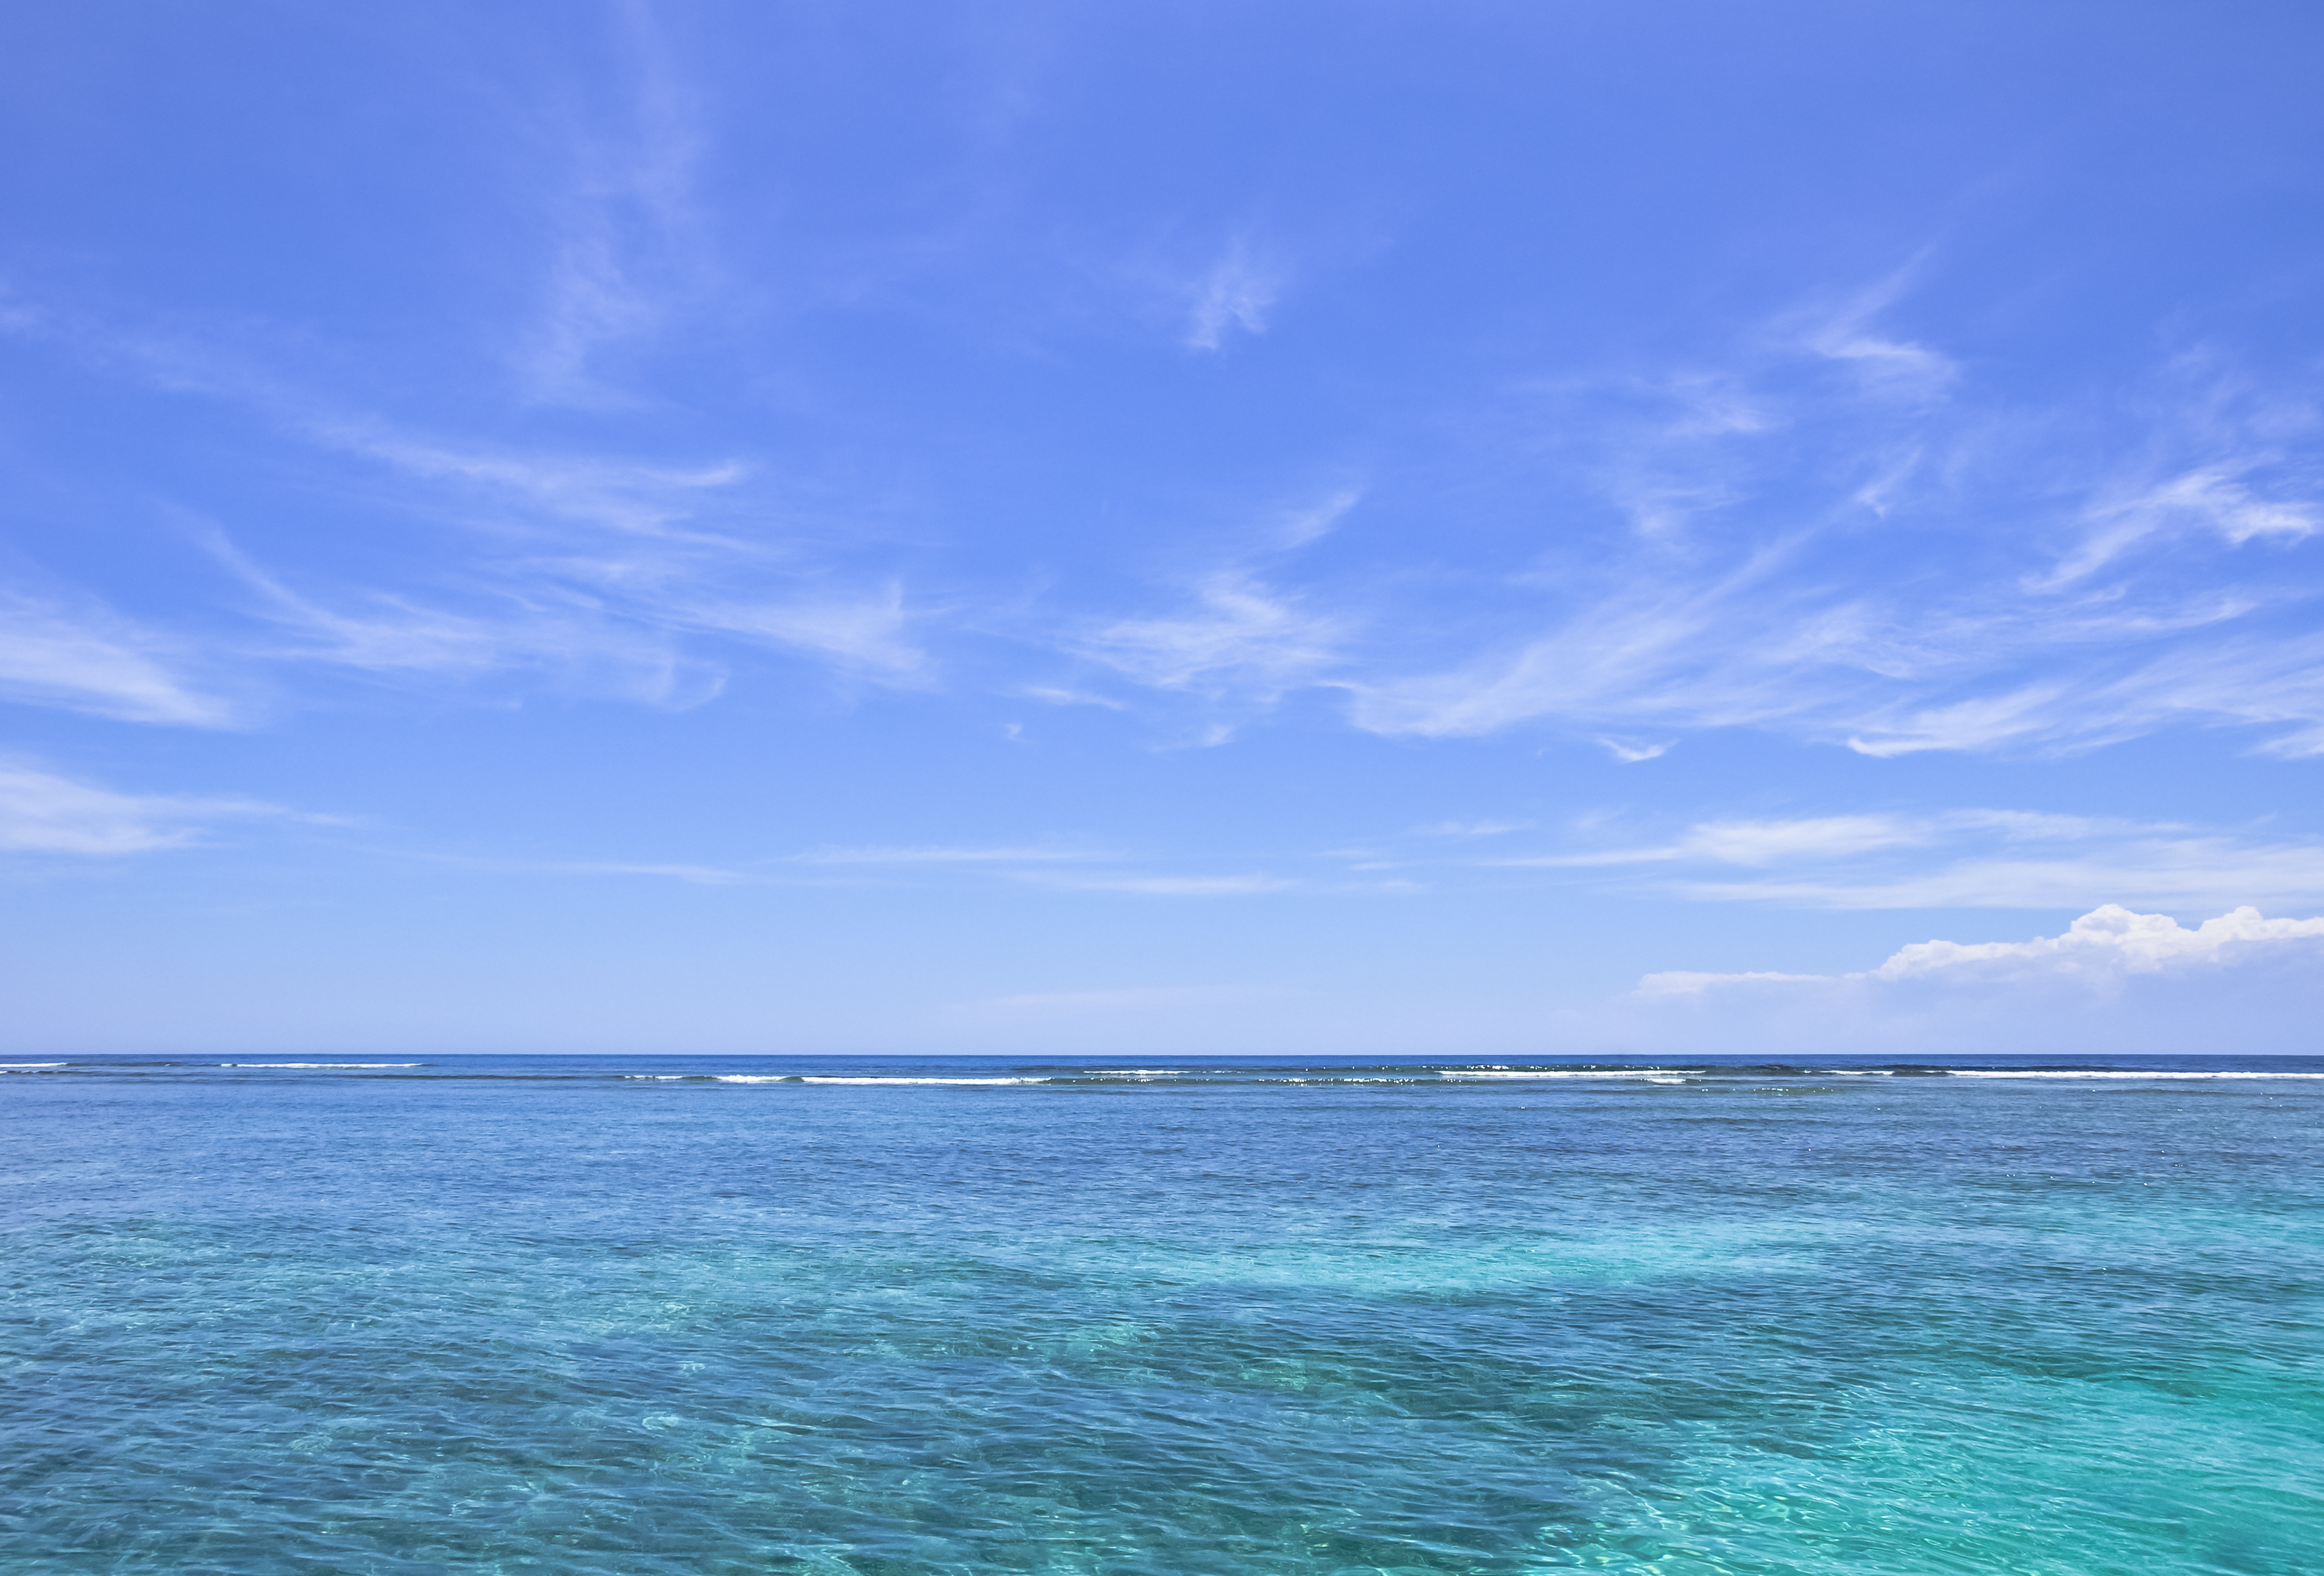
\includegraphics[width=5cm]{../1_BasicImageProcessing/output/sea.jpg}
		\vspace{-1cm}
		\renewcommand{\figurename}{Fig}
		\caption{Sea}
		\label{sea}
	\end{minipage}
	\begin{minipage}{0.5\hsize}
		\centering
		\includegraphics[width=5cm]{../1_BasicImageProcessing/output/sakura.jpg}
		\vspace{-1cm}
		\renewcommand{\figurename}{Fig}
		\caption{Sakura}
		\label{sakura}
	\end{minipage}
\end{figure}

\begin{figure}[ht]
	\begin{minipage}{0.5\hsize}
		\centering
		\includegraphics[width=5cm]{../1_BasicImageProcessing/output/sea_hist.jpg}
		\renewcommand{\figurename}{Fig}
		\caption{Sea Histgram}
		\label{sea_hist}
	\end{minipage}
	\begin{minipage}{0.5\hsize}
		\centering
		\includegraphics[width=5cm]{../1_BasicImageProcessing/output/sakura_hist.jpg}
		\renewcommand{\figurename}{Fig}
		\caption{Sakura Histgram}
		\label{sakura_hist}
	\end{minipage}
\end{figure}

\subsubsection{SURF}
Fig\ref{tomato}のトマト,Fig\ref{cucumber}のキュウリの画像に関して,SURFを用いて特徴量抽出を行った.実装はOpenCVを利用した.その結果が,Fig\ref{tomato_surf},Fig\ref{cucumber_surf}である.丸で囲まれた部分が特徴として抽出した部分を表している.

トマトの画像のSURFにより抽出された特徴は,背景の白色の部分では全くなく,トマト本体,輪郭,ヘタの部分などの多くの特徴が抽出できていることがわかる.キュウリも同様に,キュウリ本体付近から多くの特徴を抽出できている.\\

\begin{figure}[ht]
	\begin{minipage}{0.5\hsize}
		\centering
		\includegraphics[width=5cm]{../1_BasicImageProcessing/output/tomato.jpg}
		\vspace{-1cm}
		\renewcommand{\figurename}{Fig}
		\caption{Tomato}
		\label{tomato}
	\end{minipage}
	\begin{minipage}{0.5\hsize}
		\centering
		\includegraphics[width=5cm]{../1_BasicImageProcessing/output/cucumber.jpg}
		\vspace{-1cm}
		\renewcommand{\figurename}{Fig}
		\caption{Cucumber}
		\label{cucumber}
	\end{minipage}
\end{figure}

\begin{figure}[ht]
	\begin{minipage}{0.5\hsize}
		\centering
		\includegraphics[width=5cm]{../1_BasicImageProcessing/output/tomato_surf.jpg}
		\vspace{-1cm}
		\renewcommand{\figurename}{Fig}
		\caption{Tomato SURF}
		\label{tomato_surf}
	\end{minipage}
	\begin{minipage}{0.5\hsize}
		\centering
		\includegraphics[width=5cm]{../1_BasicImageProcessing/output/cucumber_surf.jpg}
		\vspace{-1cm}
		\renewcommand{\figurename}{Fig}
		\caption{Cucumber SURF}
		\label{cucumber_surf}
	\end{minipage}
\end{figure}

\section{Medical Image Classification}
VGG-16で,約91.7\%の認識率であった.AlexNetでも90\%以上の認識率を達成することができた.Fig\ref{VGG16},Fig\ref{AlexNet}に示すように,VGG16は,AlexNetよりも精度が良く,収束も早いが,1イテレーションあたりの時間が10倍ほどかかる.

\begin{figure}[ht]
	\centering
	\includegraphics[width=10cm]{../2_MedicalImageClassification/Model/VGG16_acc.png}
	\vspace{-0.5cm}
	\renewcommand{\figurename}{Fig}
	\caption{VGG16}
	\label{VGG16}
\end{figure}

\begin{figure}[ht]
	\centering
	\includegraphics[width=10cm]{../2_MedicalImageClassification/Model/AlexNet_acc.png}
	\vspace{-0.5cm}
	\renewcommand{\figurename}{Fig}
	\caption{AlexNet}
	\label{AlexNet}
\end{figure}

VGG-16,AlexNetのモデルは,ライブラリKerasを用いて,実装した.その際,参考にした論文はそれぞれ,ImageNet Classification with Deep Convolutional Neural Networks(https://arxiv.org/pdf/1409.1556.pdf),Very Deep Convolutional Networks for Large-Scale Image Recognition(https://arxiv.org/pdf/1409.1556.pdf)である.\\

VGG-16モデルを用いた認識について考察する.混合行列をTab\ref{cm}に示す.

\begin{table}[ht]
	\centering
	\renewcommand{\tablename}{Tab}
	\caption{Confusion Matrix}
	\vspace{0.5cm}
	\begin{tabular}{cc|c|c|}
	\cline{3-4}
	                                              &          & \multicolumn{2}{c|}{Predicted} \\ \cline{3-4} 
	                                              &          & Negative       & Positive      \\ \hline
	\multicolumn{1}{|c|}{\multirow{2}{*}{Actual}} & Negative & 1115           & 80            \\ \cline{2-4} 
	\multicolumn{1}{|c|}{}                        & Positeve & 123            & 1140          \\ \hline
	\end{tabular}
	\label{cm}
\end{table}

陽性の画像に関して,陰性であると予想したのは,123あった.これらの間違いには,以下の3つのパターンがあった.

\begin{itemize}
	\item 同じ部位の画像のほぼ全ての誤認識
	\item コントラストが低い
	\item 原因不明
\end{itemize}

1つ目は,同じ部位の画像のほぼ全てを誤認識してしまっているパターンである.Fig\ref{wp11},Fig\ref{wp12},Fig\ref{wp13}のような例である.それぞれ同じような画像10枚ずつほど間違えている.これは,腫瘍ではなく,この部位の形,コントラスト自体が腫瘍ありと判断してしまっていると考えられる.

\begin{figure}[ht]
	\begin{minipage}{0.32\hsize}
		\centering
		\includegraphics[width=\linewidth]{../2_MedicalImageClassification/Dataset/1253.jpg}
		\vspace{-1cm}
		\renewcommand{\figurename}{Fig}
		\caption{Wrong Image Ex.1}
		\label{wp11}
	\end{minipage}
	\begin{minipage}{0.32\hsize}
		\centering
		\includegraphics[width=\linewidth]{../2_MedicalImageClassification/Dataset/1662.jpg}
		\vspace{-1cm}
		\renewcommand{\figurename}{Fig}
		\caption{Wrong Image Ex.2}
		\label{wp12}
	\end{minipage}
	\begin{minipage}{0.32\hsize}
		\centering
		\includegraphics[width=\linewidth]{../2_MedicalImageClassification/Dataset/2314.jpg}
		\vspace{-1cm}
		\renewcommand{\figurename}{Fig}
		\caption{Wrong Image Ex.3}
		\label{wp13}
	\end{minipage}
\end{figure}

2つ目は,コントラストが低く,うまく認識できていないというパターンである.Fig\ref{wp21},Fig\ref{wp22},Fig\ref{wp23}のような例である.反対に,コントラストがはっきりしている画像に関しては,正確な値は出していないが,誤認識は少ない傾向にある印象を受けた.

\begin{figure}[ht]
	\begin{minipage}{0.32\hsize}
		\centering
		\includegraphics[width=\linewidth]{../2_MedicalImageClassification/Dataset/1319.jpg}
		\vspace{-1cm}
		\renewcommand{\figurename}{Fig}
		\caption{Wrong Image Ex.4}
		\label{wp21}
	\end{minipage}
	\begin{minipage}{0.32\hsize}
		\centering
		\includegraphics[width=\linewidth]{../2_MedicalImageClassification/Dataset/1563.jpg}
		\vspace{-1cm}
		\renewcommand{\figurename}{Fig}
		\caption{Wrong Image Ex.5}
		\label{wp22}
	\end{minipage}
	\begin{minipage}{0.32\hsize}
		\centering
		\includegraphics[width=\linewidth]{../2_MedicalImageClassification/Dataset/2006.jpg}
		\vspace{-1cm}
		\renewcommand{\figurename}{Fig}
		\caption{Wrong Image Ex.6}
		\label{wp23}
	\end{minipage}
\end{figure}

3つ目は,原因不明のパターンである.医学知識がない私では見分けがつかないような,ほぼ同じ画像が数枚ある中で,1枚だけ間違えるというものがいくつかあった.どの部分の特徴を抽出して間違えたかなど推測できなかった.

1,2つ目のパターンの間違いは,各部位ごとで学習することで,精度の向上の可能性があると考えた.理由としては,部位の形,コントラストがすべての学習データセットで等しくなり,腫瘍部分の特徴が多く抽出されると考えるからだ.しかし,問題点もある.学習に使用する画像が少ないことである.さらなるデータの収集,反転や回転による学習データの水増しなどが必要であろう.\\

陰性の画像に関して,陽性であると予想したのは,80あった.これらの間違いには,上記のの3つのパターンにプラスして,医学知識がない私が見る限りでは腫瘍らしいものが含まれている画像の誤認識というパターンがあった.Fig\ref{wp31},Fig\ref{wp32},Fig\ref{wp33}のような例である.

\begin{figure}[ht]
	\begin{minipage}{0.32\hsize}
		\centering
		\includegraphics[width=\linewidth]{../2_MedicalImageClassification/Dataset/8.jpg}
		\vspace{-1cm}
		\renewcommand{\figurename}{Fig}
		\caption{Wrong Image Ex.7}
		\label{wp31}
	\end{minipage}
	\begin{minipage}{0.32\hsize}
		\centering
		\includegraphics[width=\linewidth]{../2_MedicalImageClassification/Dataset/83.jpg}
		\vspace{-1cm}
		\renewcommand{\figurename}{Fig}
		\caption{Wrong Image Ex.8}
		\label{wp32}
	\end{minipage}
	\begin{minipage}{0.32\hsize}
		\centering
		\includegraphics[width=\linewidth]{../2_MedicalImageClassification/Dataset/106.jpg}
		\vspace{-1cm}
		\renewcommand{\figurename}{Fig}
		\caption{Wrong Image Ex.9}
		\label{wp33}
	\end{minipage}
\end{figure}

この誤認識のパターンを修正するような特徴を抽出するようなモデルを考えたとしても,今回認識できていた腫瘍ありの画像も腫瘍なしとして認識してしまう可能性が高くなると考える.今回は,腫瘍がない画像について,腫瘍ありと判断する分に関しては,大きな問題とはならないと考え,そのままとしておくほうが良いであろう.


\section{Time Series Classification}
level1~level4どれも,DTW(Dynamic Time Warping)を距離尺度とし,k-NN(k-Nearest Neighbor)を用いて識別を行った.level1ではライブラリsklearnを用いて実装したが,level2以降は,時系列データは,高次元,可変長であるため,DTW計算は,ライブラリtslearnを用いて計算を行い,k-NNは自ら実装した.DTW距離(Wraping Path)の計算の際の動的計画法を適用する行列の各要素は,時系列データの各点同士のL2ノルムの2乗を採用している.
level1~level3の全てで認識率100\%を達成することができた.同じ方法で,level4は,referenceフォルダのデータを教師データ用,validationデータ用に,2:1で分け,テストしたところ,認識率100\%を得ることができた.testデータに対しては,data1.datから順に,1, 1, 1, 1, 1, 1, 1, 2, 2, 2, 2, 2, 1, 2と予想された.

\end{document}




















